\vspace{-7mm}
\begin{minipage}{0.45\textwidth}
    \begin{IEEEbiography}[{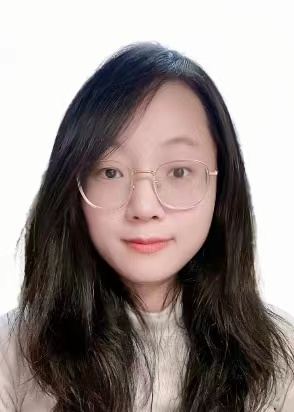
\includegraphics[width=1in,height=1.25in,clip,keepaspectratio]{Photos/xueli_sun.jpeg}}]{Xueli Sun}
         received the Ph.D. degree in computer science from Soochow University, Suzhou, China. She is currently a Lecturer with the School of Internet of Things, Nanjing University of Posts and Telecommunications. Her current research interests include interconnection architectures, data center networks, fault diagnosis, network reliability, and graph learning.
    \end{IEEEbiography}
\end{minipage}
\vspace{-5mm}
\begin{minipage}{0.45\textwidth}
    \begin{IEEEbiography}[{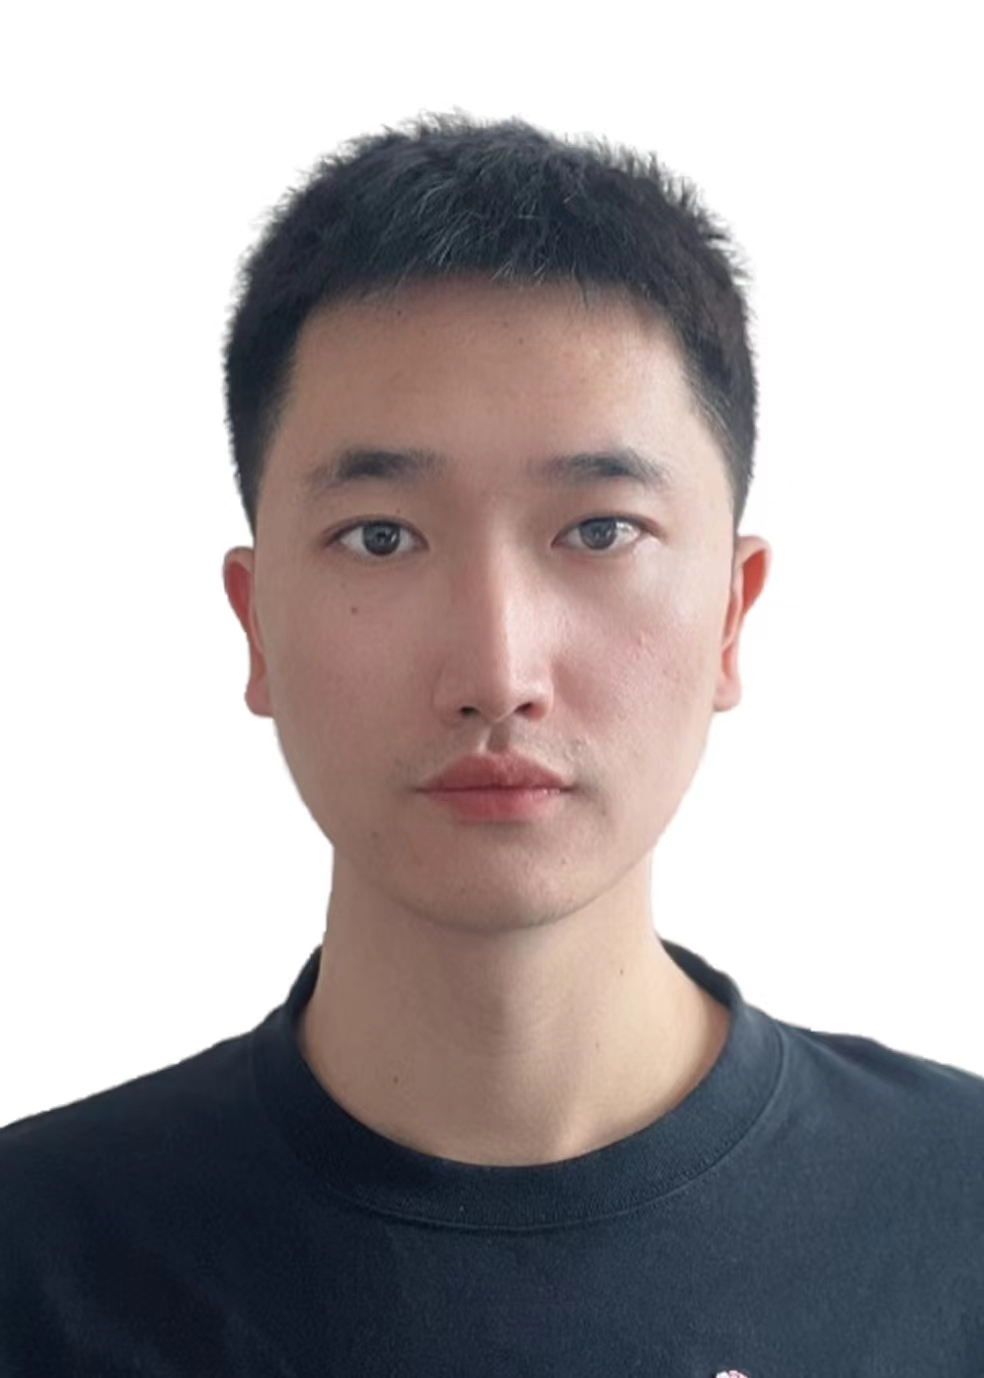
\includegraphics[width=1in,height=1.25in,clip,keepaspectratio]{Photos/shuangxiang_kan.jpeg}}]{Shuangxiang Kan}
        received the M.Sc. degree from Soochow University, in 2021. He is currently working toward the Ph.D. degree with the University of New South Wales. His current research interests include static and dynamic program analysis, program verification, and interconnection architectures.
    \end{IEEEbiography}
\end{minipage}
\vspace{-5mm}
\begin{minipage}{0.45\textwidth}
    \begin{IEEEbiography}[{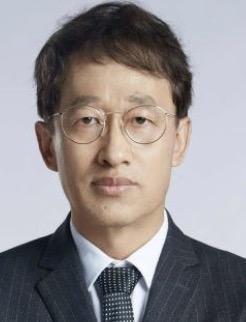
\includegraphics[width=1in,height=1.25in,clip,keepaspectratio]{Photos/jianxi_fan.jpeg}}]{Jianxi Fan}
        received the Ph.D. degree in computer science from the City University of Hong Kong, Hong Kong, in 2006. He is currently a Professor with the School of Computer Science and Technology, Soochow University, China.  His research interests include parallel and distributed systems, interconnection architectures, data center networks, and graph algorithms.
        % received the B.S. degree in computer science from Shandong Normal University, Jinan, in 1988, the M.S. degree in computer science from Shandong University, Jinan, in 1991, and the Ph.D. degree in computer science from the City University of Hong Kong, Hong Kong, in 2006. He is currently a Professor with the School of Computer Science and Technology, Soochow University, China.  His research interests include parallel and distributed systems, interconnection architectures, data center networks, and graph algorithms.
    \end{IEEEbiography}
\end{minipage}
\vspace{-5mm}
\begin{minipage}{0.45\textwidth}
    \begin{IEEEbiography}[{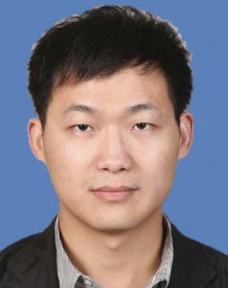
\includegraphics[width=1in,height=1.25in,clip,keepaspectratio]{Photos/weibei-fan.jpeg}}]{Weibei Fan}
        (Member, IEEE) received the Ph.D. degree in computer science from Soochow University, in 2019. He is currently an Associate Professor with the School of Computer, Nanjing University of Posts and Telecommunications. His research interests include data centers, parallel and distributed systems, and interconnection architectures.
    \end{IEEEbiography}
\end{minipage}
\vspace{-5mm}
\begin{minipage}{0.45\textwidth}
    \begin{IEEEbiography}[{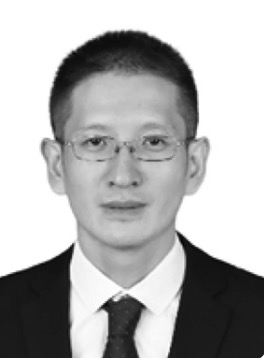
\includegraphics[width=1in,height=1.25in,clip,keepaspectratio]{Photos/jin_qi.jpeg}}]{Jin Qi}
        (Member, IEEE) received the Ph.D. degrees in information network from Nanjing University of Posts and Telecommunications, Nanjing, China, in 2012. He is currently a Professor with the School of Internet of Things in Nanjing University of Posts and Telecommunications. His main research interests are in the areas of intelligent computing, industrial Internet, and energy Internet.
    \end{IEEEbiography}
\end{minipage}
\vspace{-5mm}
\begin{minipage}{0.45\textwidth}
    \begin{IEEEbiography}[{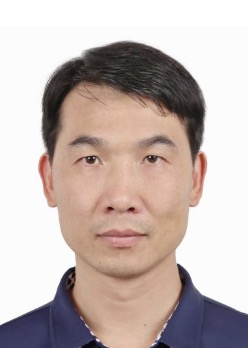
\includegraphics[width=1in,height=1.25in,clip,keepaspectratio]{Photos/zhenjiang_dong.jpeg}}]{Zhenjiang Dong}
         received the Ph.D. degree from Shanghai Jiao Tong University, Shanghai, China. He is currently a Full Professor with the School of Computer Science, Nanjing University of Posts and Telecommunications. His current research interests include security of data element flows, privacy computing, cyberspace security, and blockchain.
    \end{IEEEbiography}
\end{minipage}
